\documentclass{prova}

\usepackage{amsmath}
\usepackage{amsfonts}

\setlength{\textwidth}{18cm}
\setlength{\textheight}{27cm}
\setlength{\topmargin}{-2.3cm}
\setlength{\oddsidemargin}{-1cm}

\renewcommand{\sin}{\,\mbox{sen}\,}
\newcommand{\ds}{\displaystyle}

%\hyphenation{cor-res-pon-d\^en-ci-as}

\professor{Prof.\@ Adriano Barbosa}
\disciplina{C\'alculo de V\'arias Vari\'aveis}
\avaliacao{PS}
\curso{Matem\'atica}
\data{26/04/2023}

\begin{document}
	\cabecalho{5}  % o numero 5 indica a qnt de quadros na tabela de nota

    \textbf{Todas as respostas devem ser justificadas.}

    \vspace{0.5cm}
    \textbf{Avalia\c{c}\~ao P1:}
    \begin{questionario}
        \q{Determine a correspond\^encia entre as fun\c{c}\~oes e seus gr\'aficos (A, B
           e C). Em seguida, determine a correspond\^encia entre os gr\'aficos e
           as curvas de n\'{\i}vel (I, II e III)}
           \begin{questionariol}
               \ql{$z=\sin(xy)$}
               \ql{$z=e^x \cos y$}
               \ql{$z=(1-x^2)(1-y^2)$}
           \end{questionariol}
           \begin{figure}[h]
               \centering
               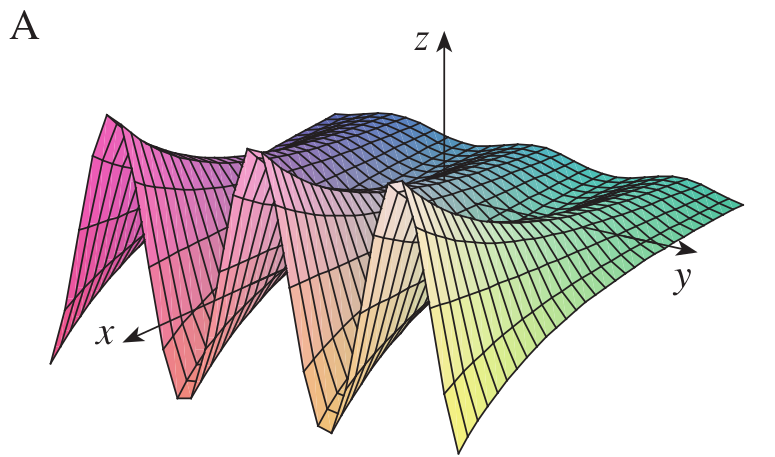
\includegraphics[width=0.3\textwidth]{p1-q1-1.png}
               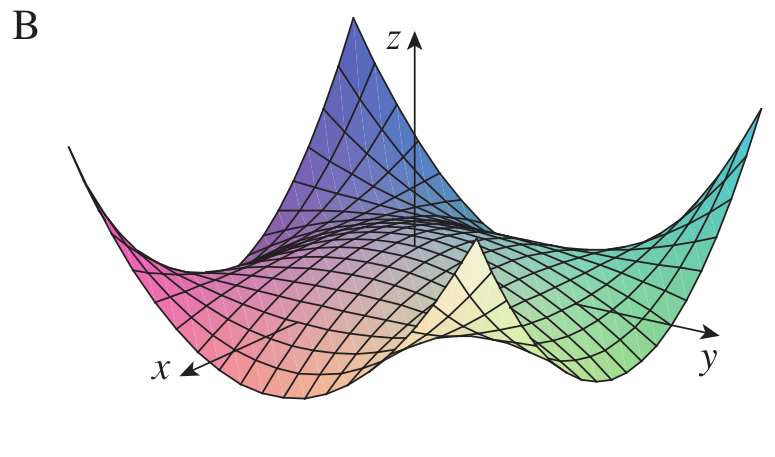
\includegraphics[width=0.3\textwidth]{p1-q1-2.png}
               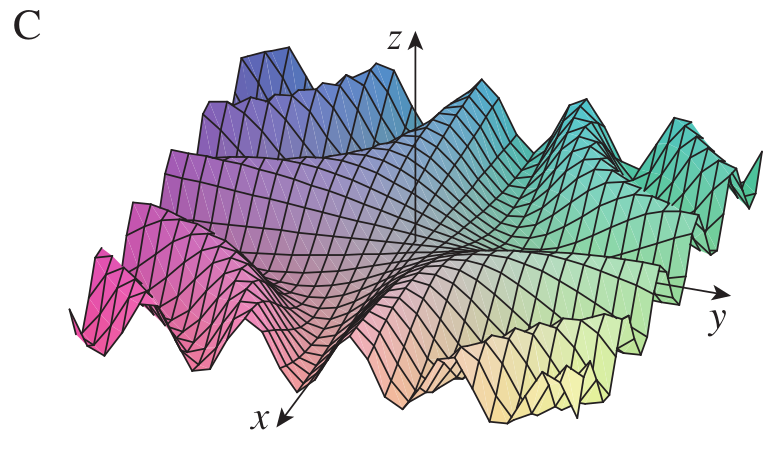
\includegraphics[width=0.3\textwidth]{p1-q1-3.png}
               \\
               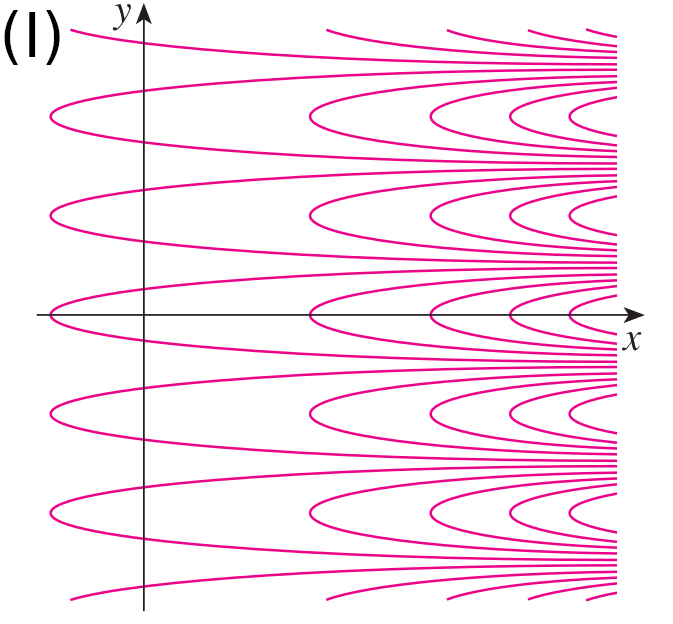
\includegraphics[width=0.3\textwidth]{p1-q1-a.png}
               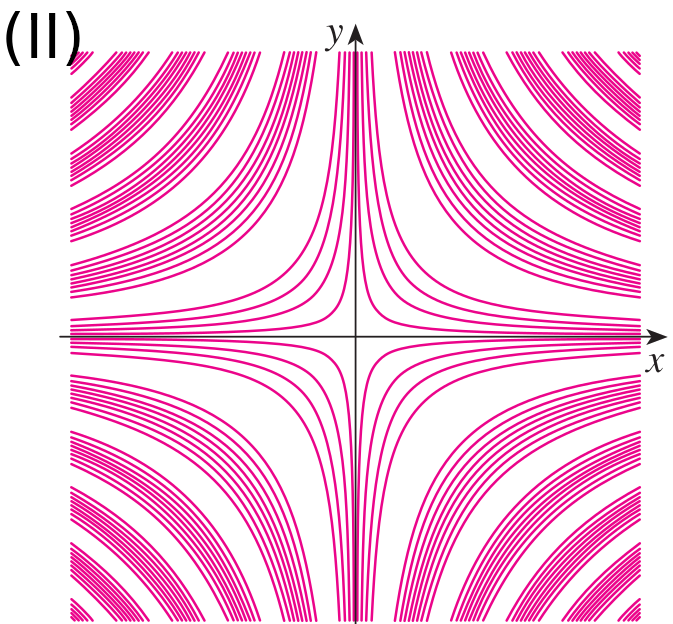
\includegraphics[width=0.3\textwidth]{p1-q1-b.png}
               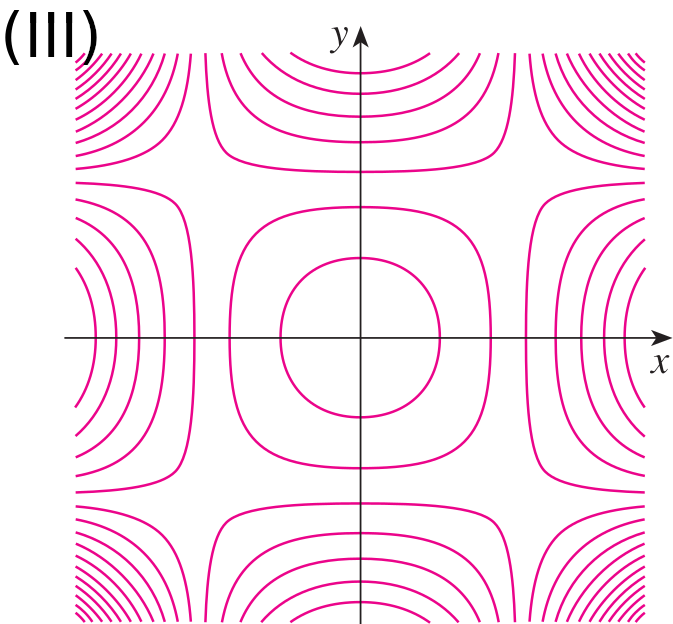
\includegraphics[width=0.3\textwidth]{p1-q1-c.png}
           \end{figure}
        \q{Calcule os limites abaixo:}
            \vspace{0.2cm}
            \begin{questionariol}
                \ql{$\ds\lim_{(x,y)\rightarrow(0,0)}
                    \frac{x^4-4y^2}{x^2+2y^2}$}
                \ql{$\ds\lim_{(x,y)\rightarrow(0,0)}
                    \frac{xy}{\sqrt{x^2+y^2}}$}
            \end{questionariol}
        \q{Encontre a taxa de varia\c{c}\~ao m\'axima de $f(x,y)=x^2y+\sqrt{y}$ no
           ponto $(2,1)$. Em que dire\c{c}\~ao ela ocorre?}
        \q{Se $u=x^2y^3+z^4$, onde $x=p+3p^2$, $y=pe^p$ e $z=p\sin p$, use a
           regra da cadeia para calcular $\ds\frac{du}{dp}$.}
        \q{Encontre os valores m\'aximo e m\'{\i}nimo local e pontos de sela da
           fun\c{c}\~ao $f(x,y)=x^2-xy+y^2+9x-6y+10$.}
    \end{questionario}

    \newpage{}
    \vspace{0.5cm}
    \textbf{Avalia\c{c}\~ao P2:}
    \begin{questionario}
        \q{Determine se as afirma\c{c}\~oes s\~ao verdadeiras ou falsas. Justifique as
           verdadeiras e d\^e um contra-exemplo para as falsas.}
           \begin{questionario}
               \qq{$\ds\int_{-1}^2\int_0^6 x^2\sin(x-y)\ dxdy =
                   \int_0^6\int_{-1}^2 x^2\sin(x-y)\ dydx$.}
                \qq{$\ds\int_1^2\int_3^4 x^2 e^y\ dydx = \int_1^2 x^2\
                    dx\int_3^4 e^y\ dy$.}
                \qq{Se $f$ \'e cont\'{\i}nua em $[0,1]$, ent\~ao $\ds\int_0^1\int_0^1
                    f(x)f(y)\ dydx = \left[\int_0^1 f(x)\ dx\right]^2$}
           \end{questionario}
        \q{Calcule a integral $\ds\iint_D \frac{y}{1+x^2}\ dA$, onde $D$ \'e
           limitada pelas curvas $y=\sqrt{x}$, $y=0$ e $x=1$.}
        \q{Use coordenadas polares para determinar o valor da integral
           $\ds\int_0^3\int_{-\sqrt{9-x^2}}^{\sqrt{9-x^2}} (x^3+xy^2)\ dydx$.}
        \q{Reescreva a integral $\ds\int_{-1}^1\int_{x^2}^1\int_0^{1-y}
           f(x,y,z)\ dzdydx$ como uma integral iterada na ordem $dxdydz$.}
        \q{Use coordenadas esf\'ericas para calcular
           $\ds\int_{-2}^2\int_0^{\sqrt{4-y^2}}\int_{-\sqrt{4-x^2-y^2}}^{\sqrt{4-x^2-y^2}}
           y^2\sqrt{x^2+y^2+z^2}\ dzdxdy$.}
    \end{questionario}
\end{document}
